\subsection{Einführung}
Der Grund für die Entwicklung von LTE liegt in der immer steigenden nachfrage nach Mobilkommunikation und im speziellen nach Mobilem Internet. Zudem ist die Anzahl der Subscriber stetig am steigen. Auch die steigende Verbreitung der Smartphones führt zur erhöhten nachfrage, welche mit UMTS / HSDPA nicht mehr abgedeckt werden konnte. \\
\subsubsection{Ziele von LTE}
Das Ziel von LTE war, einen Downlink von mindestens 100 Mbps und ein Uplink von mindestens 50 Mbps zu erreichen. Zudem wurde eine Round-Trip-Zeit von wengier als 10 ms angepeilt. Das System sollte für Packet Switched optimiert werden und eine höhere Mobilität und Sicherheit als bisherige Standards bieten. Auch die Zellen grösse die Typisch 5-30 km sein sollten, aber über 100 km möglich sein sollten, waren nicht mehr gleich wie bei Vorgängern. Die Flexibilität der Frequenz sollte erreicht werden, mit einer neuer Codierung. Als Protokoll war das IP Multimedia Subsystem (IMS) vorgesehen.

\subsubsection{Hauptänderungen zu UMTS}
Die Codierung wurde von WCDMA (Wideband Code Division Multiple Access)auf OFDMA (Orthogonal Frequency-Division Multiple Access)umgestellt. Dies hat die Probleme mit Multifading gelöst. Man hat viele langsame Subcarrier, die aber in ihrer Datenrate konstant bleiben. \\
MIMO (Multiple Input Multiple Output) erlaubt die gleichzeitige Übertragung mehrerer Datenströme über einen Kanal.\\
IP (Internet Protocol): Neu lag der Fokus definitiv auf das paketvermittelnde Kernnetz. Einzige Ausnahme ist SMS das auch weiterhin über die Signalisierungsnachrichten abgewickelt werden. \\
Defninition von QoS (Qualitiy of Service)  Mechanismen welche vorallem bei erreichen der Kapazitätsgrenzen wichtig wird. \\
Mit der Vereinfachung des Netzwerks konnte die Round-Trip-Delay-Zeit unter 30 ms gebracht werden. \\
Ein weiter Punkt war der Fokus auf Multimode Endgeräte, welche neben LTE auch GSM, GPRS, EDGE, UMTS, HSPA unterstützten, was ein geeignetes Protokoll benötigt.


\subsubsection{Stand der Technik}
Der Stand der Technik ist, dass LTE momentan bei verschiedenen Providern im Aufbau ist. In viel bevölkerten Regionen ist LTE heute schon Realität. Im LTE Advanced, dem Nachfolger von LTE sind theoretisch 1 Gbps möglich. Dieser Standard ist zwar verabschiedet aber noch nicht verbreitet.

\subsection{LTE Architektur und Protokolle}
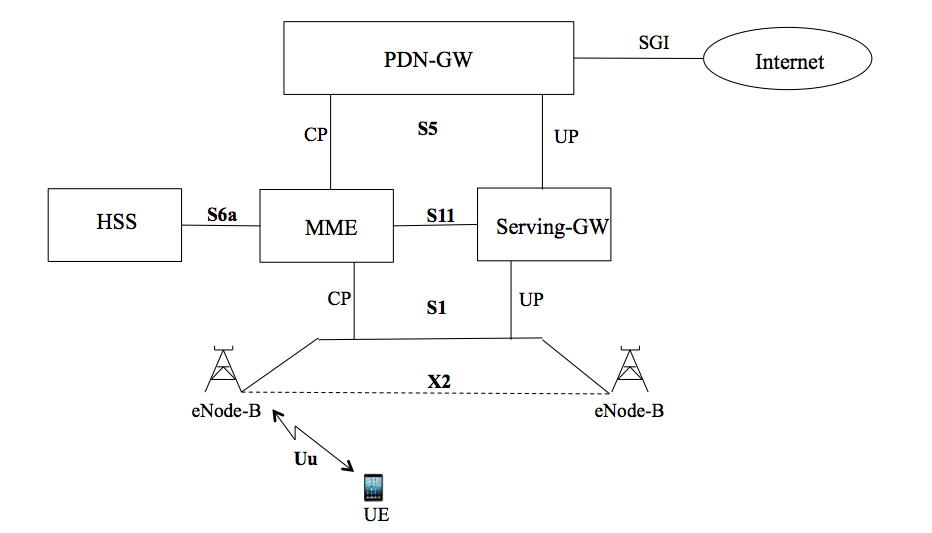
\includegraphics[width = 0.5 \linewidth]{./Pics/LTE1.png}
\subsubsection{UE User Equipment }
Das UE bezeichnet das Endgerät. Hier hat sich bezüglich UMTS geändert, dass neu eine LTE spezifische SIM Card verwendet werden muss, USIM (Universal Subscriber Identity Modul). Diese USIM dient zur Authentifizierung des Benutzers und zur Ableitung der Sicherheitsschlüssel zum Schutz der Funkschnittstelle. Jedes UE hat nur eine Verbindung zu heweils einem eNB. \\
Das UE muss folgende dinge erledigen. Ciphering/deciphering von User Plane (UP) Daten, IP header compression/decompression sowie das erstellen von Messberichten. 

\subsubsection{eNodeB und S1/X2 Schnittstellen}
Der Name eNodeB leitet sich vom Node B in UMTS ab. (e = evolved). Dieser ersetzt die in UMTS verwendeten Komponenten NodeB und RNCNode. Der eNodeB führt selbständig Handover-Prozeduren durch und informiert das Corenet erst danach. Der eNodeB ist ebenfalls für die Auswertung der Messberichten und das Interferenzenmanagement verantwortlich. \\
Die Schnittstelle zum Kernnetz wird als S1 bezeichnet. \\ 
Ein eNodeB besteht aus, Antenne, Radiomodul, Digitalmodul, Anbindung an das Kernnetz über IP-basiertes Backhaul sowie Verbindung zu benachbarten eNodeBs via X-Interface. \\ \\
S1 CP Control Plane: \\
Wird zur Signalisierung verwendet. Es werden mehrere Signalisierungsstreams gleichzeitig versandt. Hierzu wird nicht mehr TCP sonder SCTP verwendet (Stream Control Transmission Protocol). SCTP ist verantwortlich für Flusskontrolle, Reihenfolgekontrolle und für Überlastungsmanagement. \\
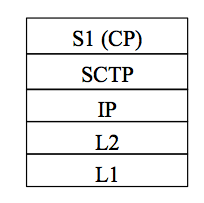
\includegraphics[width = 0.2 \linewidth]{./Pics/LTE2.png} 
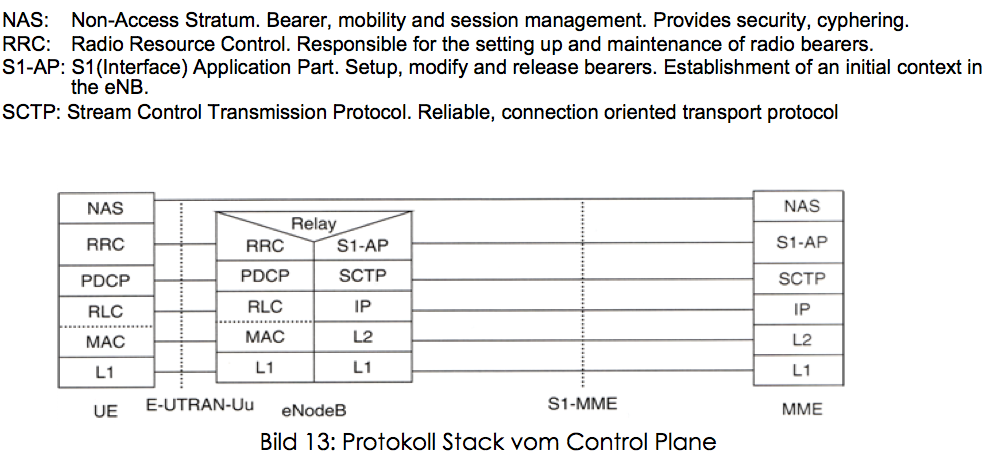
\includegraphics[width = 0.75 \linewidth]{./Pics/LTE5.png}\\
S1 UP User Plane : \\
Überträgt die Nutzdaten ähnlich wie bei GPRS und legt den Tunnel des GTp um bei einem Handover. Die Schichten L1 und L2 sind nicht weiter Standardisiert und deshalb können hier verschiedene Protokolle zum Einsatz kommen. \\
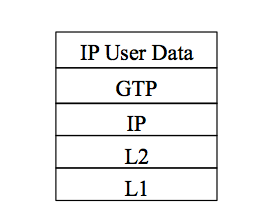
\includegraphics[width = 0.2 \linewidth]{./Pics/LTE3.png} 
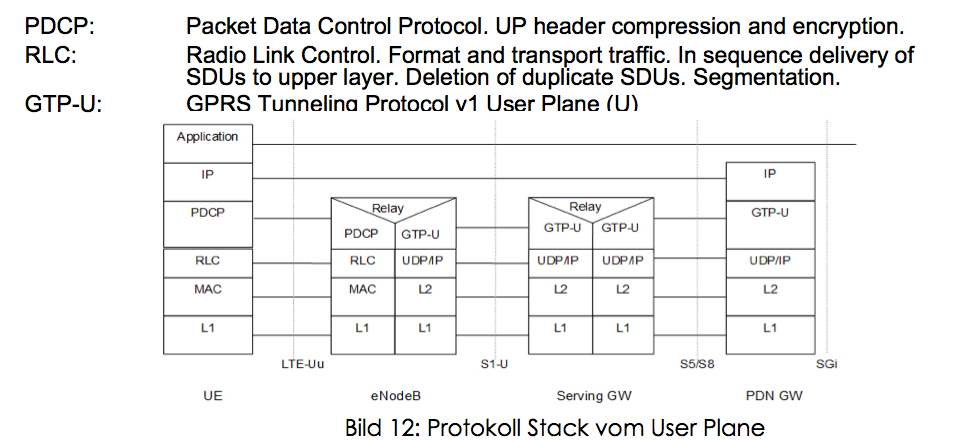
\includegraphics[width = 0.75 \linewidth]{./Pics/LTE4.png} \\
\subsubsection{MME Mobility Management Entity}
Die MME ist für die Benutzerverwaltung zuständig, dies auch wenn der eNodeB einen Teil davon schon erledigt. Der MME führt mit der HSS Home Subscriber Server eine zentrale Nuterdatenbank. In grossen Netzen können mehrere MME erforderlich sein. Die MME gehören zum Non-Access-Stratum. Die Hauptaufgaben des MME ist, die Authentisierung bevor Daten ausgetauscht werden können. Der MME kommuniziert mit dem eNodeB und fordert alle erforderlichen Daten vom HSS an. Nach der Authentisierung verschlüsselt das MME die Kommunikation. \\
Eine weiter Aufgabe ist das Aufbauen von Bearern welche die Übertragungskapazität in den Tunnels bereitstellt. Für das ist die Kommunikation zwischen Knoten nötig. Es werden Tunnel zwischen eNodeB und Netzwerken wie z.B. PDN oder dem Internet hergestellt. \\
Auch das NAS Management ist Teilaufgabe des MME.
Mit dem NAS (Non Access Stratum) Management ist gemeint, dass bei Inaktivität eines Nutzers die Deaktivierung von logischen Tunnels und der Drahtlosenschnitstelle gemacht wird. Im inaktiven Zustand entscheidet das UE selbständig über einen Zellenwechsel. Ist jedoch mit dem Zellwechsel auc ein wechsel der Tracking Area verbunden, so muss das MME involviert werden. \\
Kommt während der Inaktivität Daten für ein UE an, so wird über den eNodeB der letzten bekannten Tracking Area eine Paging-Nachricht gesant. Auf diese Nachricht muss sich das UE melden. \\
Findet ein Handover zwischen zwei eNodeBs statt die nicht über die X-Schnittstelle verbunden sind so erfolgt die Koordination über das MME. \\ 
Das selbe gilt, wenn ein Handover in ein anderes RAN (Radio Access NEtworks) wie GSM/GPRS,EDGE oder UMTS stattfindet. Auch hier muss das MME die Koordination übernehmen. \\
Auf den ersten Blick ist das MME das selbe wie das SGSN im UMTS doch ist das MME nur für die Signalisierung zuständig. Für die Weiterleitung der Nutzerdaten ist das Serving-Gateway(S-GW) zuständig.

\subsubsection{S-GW - Serving-Gateway}
Das S-GW ist für das Weiterleiten von Nutzdaten in IP Tunneln zwischen eNodeBs nd dem PDN Gateway verantwortlich. Auf Radioseite terminiert das S-GW den S1 UP GTP Tunnel, auf Netzseite terminiert das S-GW den S5-UP GTP Tunnel zum Internet GW.\\ 
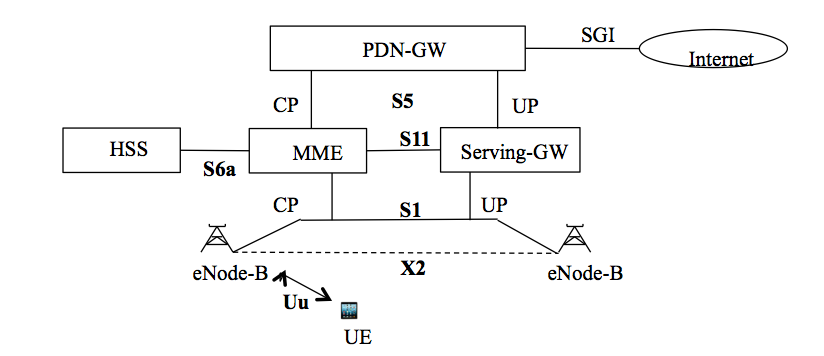
\includegraphics[width = 0.5 \linewidth]{./Pics/LTE6.png}

\subsubsection{PDN Gateway}
Der PDN Gateway ist in der Regel der Übergang zum Internet aber auch für die Anbindung von Firmennetzen über einen verschlüsselten Zugang. Der PDN Gateway vergiebt IP-Adressen an die UE. Der eNodeB fordert die MME zu Authentisierung auf, danach fordert das MME beim PDN eine IP-Adresse an.  Mit der Zuteilung einer IP werden auch die Nutzdaten Tunnel via S1 und S5 aufgebaut.

\subsubsection{HSS Home Subscriber Server}
In LTE, GSM und UMTS werden eine gemeinsame Teilnehmerdatenbank verwendet, die HSS oder auch HLR. Der unterschied liegt in der Schnittstelle zur Datenbank. Während GSM/UMTS viea Mobile Application Part (MAP Protocol) zwischen HLR und MSC und SGSN zugreifen, verwendet LTE konsequent IP basiertes Protokoll, das DIAMETER-Protokoll.
Obwohl das HLR bei LTE HSS heisst, sind sie in der praxis in der Regel identisch, so können Übergänge von einem anderen Netz einfacher realisiert werden. \\ 
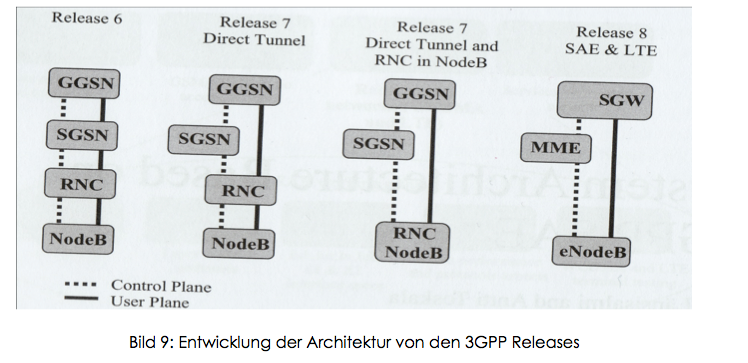
\includegraphics[width = 0.75 \linewidth]{./Pics/LTE7.png}
\subsubsection{Einbettung in das EPS: Evolved Packet System}
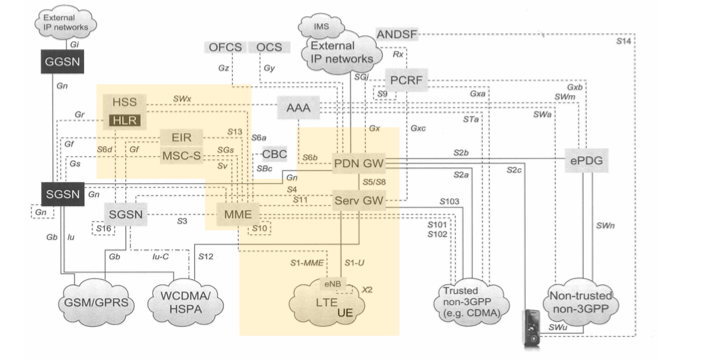
\includegraphics[width = 0.75 \linewidth]{./Pics/LTE8.png}
\subsection{Physikalische Schicht}
Wie bei den meisten modernen Funk-Technologien wird bei LTE das Orthogonal Frequency Division Multiple Access (OFDMA) Verfahren zur Modulation verwendet und zudem die Multiple Input Multiple Output (MIMO) Technologie eingesetzt. \\
Im UpLink basiert die Übertragung auf OFDM im DownLink werden verschiedene Modulationsverfahren angewendet. Hier ausschlaggebend ist die Einsparung von Energie, um den Akku des UE zu schonen. \\
OFDMA ist eine Weiterentwicklung von OFDM. Einem Benutzer können dynamisch mehrere Subcarrier zugeordnet werden. Damit wird eine optimale Bandbreitennutzung erreicht. OFDMA wird im Downlink verwendet. \\
SC-FDMA (Single Carrier Frequency Division Multiple Accesss) basiert auf dem OFDM Prinzip. 